\chapter{Metodi tradizionali}
La caratteristica degli algoritmi di compressione tradizionali è quella di usare trasformate statiche all’interno del primo blocco, messe a punto in numerosi anni di ricerca. Questa staticità non permette a questi metodi di adattarsi dinamicamente a tutti i tipi di contenuti delle immagini. Inoltre rende lo sviluppo di un nuovo algoritmo di compressione un processo lungo che richiede anni di studi e progettazione. \cite{cheng2018deep}
Andiamo ora a parlare brevemente dei metodi che andremo a considerare quando valuteremo le prestazioni dei vari algoritmi per poterli confrontare.

\section{Codifica JPEG}
Questo metodo di compressione sviluppato nel 1992 è diventato in poco tempo il formato di compressione più diffuso. Nonostante i numerosi tentativi di sostituirlo con formati più moderni questo è rimasto ancora ad oggi il formato più usato, principalmente grazie alla sua facilità implementativa. Il JPEG si basa sull’utilizzo della Discrete Cosine Transform o DCT per realizzare la rappresentazione sparsificata dell’immagine originale. I valori prodotti dall'applicazione della trasformata vengono poi quantizzati e codificati con due metodi denominati zig-zag scan e run length coding, al termine viene applicata la codifica entropica. \cite{125072} \\
Possiamo vedere un esempio di compressione con JPEG nella figura \ref{fig:CompressionJPEG}

\section{Codifica JPEG2000}
Nel 2001 con la crescente diffusione di internet, con l’aumento di dimensione e la richiesta di una maggiore qualità delle immagini, viene sviluppato questo nuovo formato chiamato appunto JPEG2000 in virtù dell'anno in cui è stato sviluppato.\\
JPEG2000 non utilizza la DCT come il suo predecessore ma viene introdotta una nuova trasformata, la DWT o Discrete Wavelet Transformat, che si propone di meglio identificare e comprimere i bordi delle figure che compongono le immagini, ovvero il dettaglio che ci permette di distinguere le varie regioni all'interno di un’immagine.
Un’ulteriore differenza di JPEG2000 è la sua capacità di comprimere le immagini con qualità progressiva, ovvero permettere di tagliare la stringa di bit in posizioni diverse per ottenere diversi livelli di qualità. Se provassimo a tagliare invece la rappresentazione in bit di JPEG, otterremo un’immagine incompleta.\\
JPEG2000 quindi voleva essere un formato di qualità superiore con una compressione più efficiente.\cite{952804}\\
Possiamo vedere un esempio di compressione con JPEG2000 nella figura \ref{fig:CompressionJPEG2000}

\section{Codifica BPG}
Il formato Better Portable Graphics è stato sviluppato da Fabrice Bellard nel 2014 con l'obbiettivo di sostituire l’ormai affermato formato JPEG. Questo metodo si basa sulla codifica intra-frame del codec HEVC o H.265 \cite{BPGImageformat}.\\
H.265 a differenza di JPEG e JPEG2000 aggiunge nuove tecniche di predizione spaziale intra-frame per comprimere ulteriormente l’immagine, queste tecniche sfruttano la ridondanza spaziale, come ad esempio le regioni omogenee. Durante la codifica le varie tecniche vengono provate e viene scelta quella migliore. Inoltre la dimensione dei blocchi in cui viene suddivisa l’immagine non è più fissa ma può variare durante la codifica.
La trasformata e la codifica entropica rimangono invece concettualmente simili ai metodi precedenti, ma utilizzano degli algoritmi più avanzati.\\
L’obbiettivo di  Bellard era quello di realizzare un formato molto leggero che potesse fornire immagini più compresse rispetto a JPEG, ma con una qualità superiore, di cui possiamo vedere un esempio nella figura \ref{fig:CompressionBPG}

\section{Codifica VVC}
Versatile Video Coding (VVC) o H.266 è lo standard di codifica video più recente, finalizzato nel luglio 2020. È stato sviluppato dal Joint Video Experts Team (JVET) dell'ITU-T Video Coding Experts Group (VCEG) e dell'ISO/IEC Moving Picture Experts Group (MPEG) per soddisfare la crescente richiesta di una migliore compressione video, per supportare una più ampia gamma di contenuti multimediali attuali e applicazioni emergenti come contenuti in High Dynamic Range (HDR), a 360°, per la Realtà Virtuale (VR) o la Realtà Aumentata (AR) \cite{9503377}.\\
Sebbene sia stato sviluppato per la compressione video, fornisce ottimi risultati anche per la compressione di immagini con metodo intra.\\
Come il suo predecessore, H.266 utilizza tecniche di predizione spaziale intra-frame e blocchi a dimensione variabile. A differenza del suo predecessore però le tecniche di predizione sono molte di più e più elaborate, e la dimensione di blocco può variare con più libertà.
La trasformata e la codifica entropica rimangono simili ai metodi precedenti, ma utilizzano degli algoritmi più avanzati.\\
L’algoritmo di codifica VVC rappresenta l’attuale stato dell’arte per la compressione di video ed immagini, ne possiamo vedere un esempio nella figura \ref{fig:CompressionVVC}
\newline

\begin{figure}[h!]
    \centering
    \begin{subfigure}[]{0.3\textwidth}
        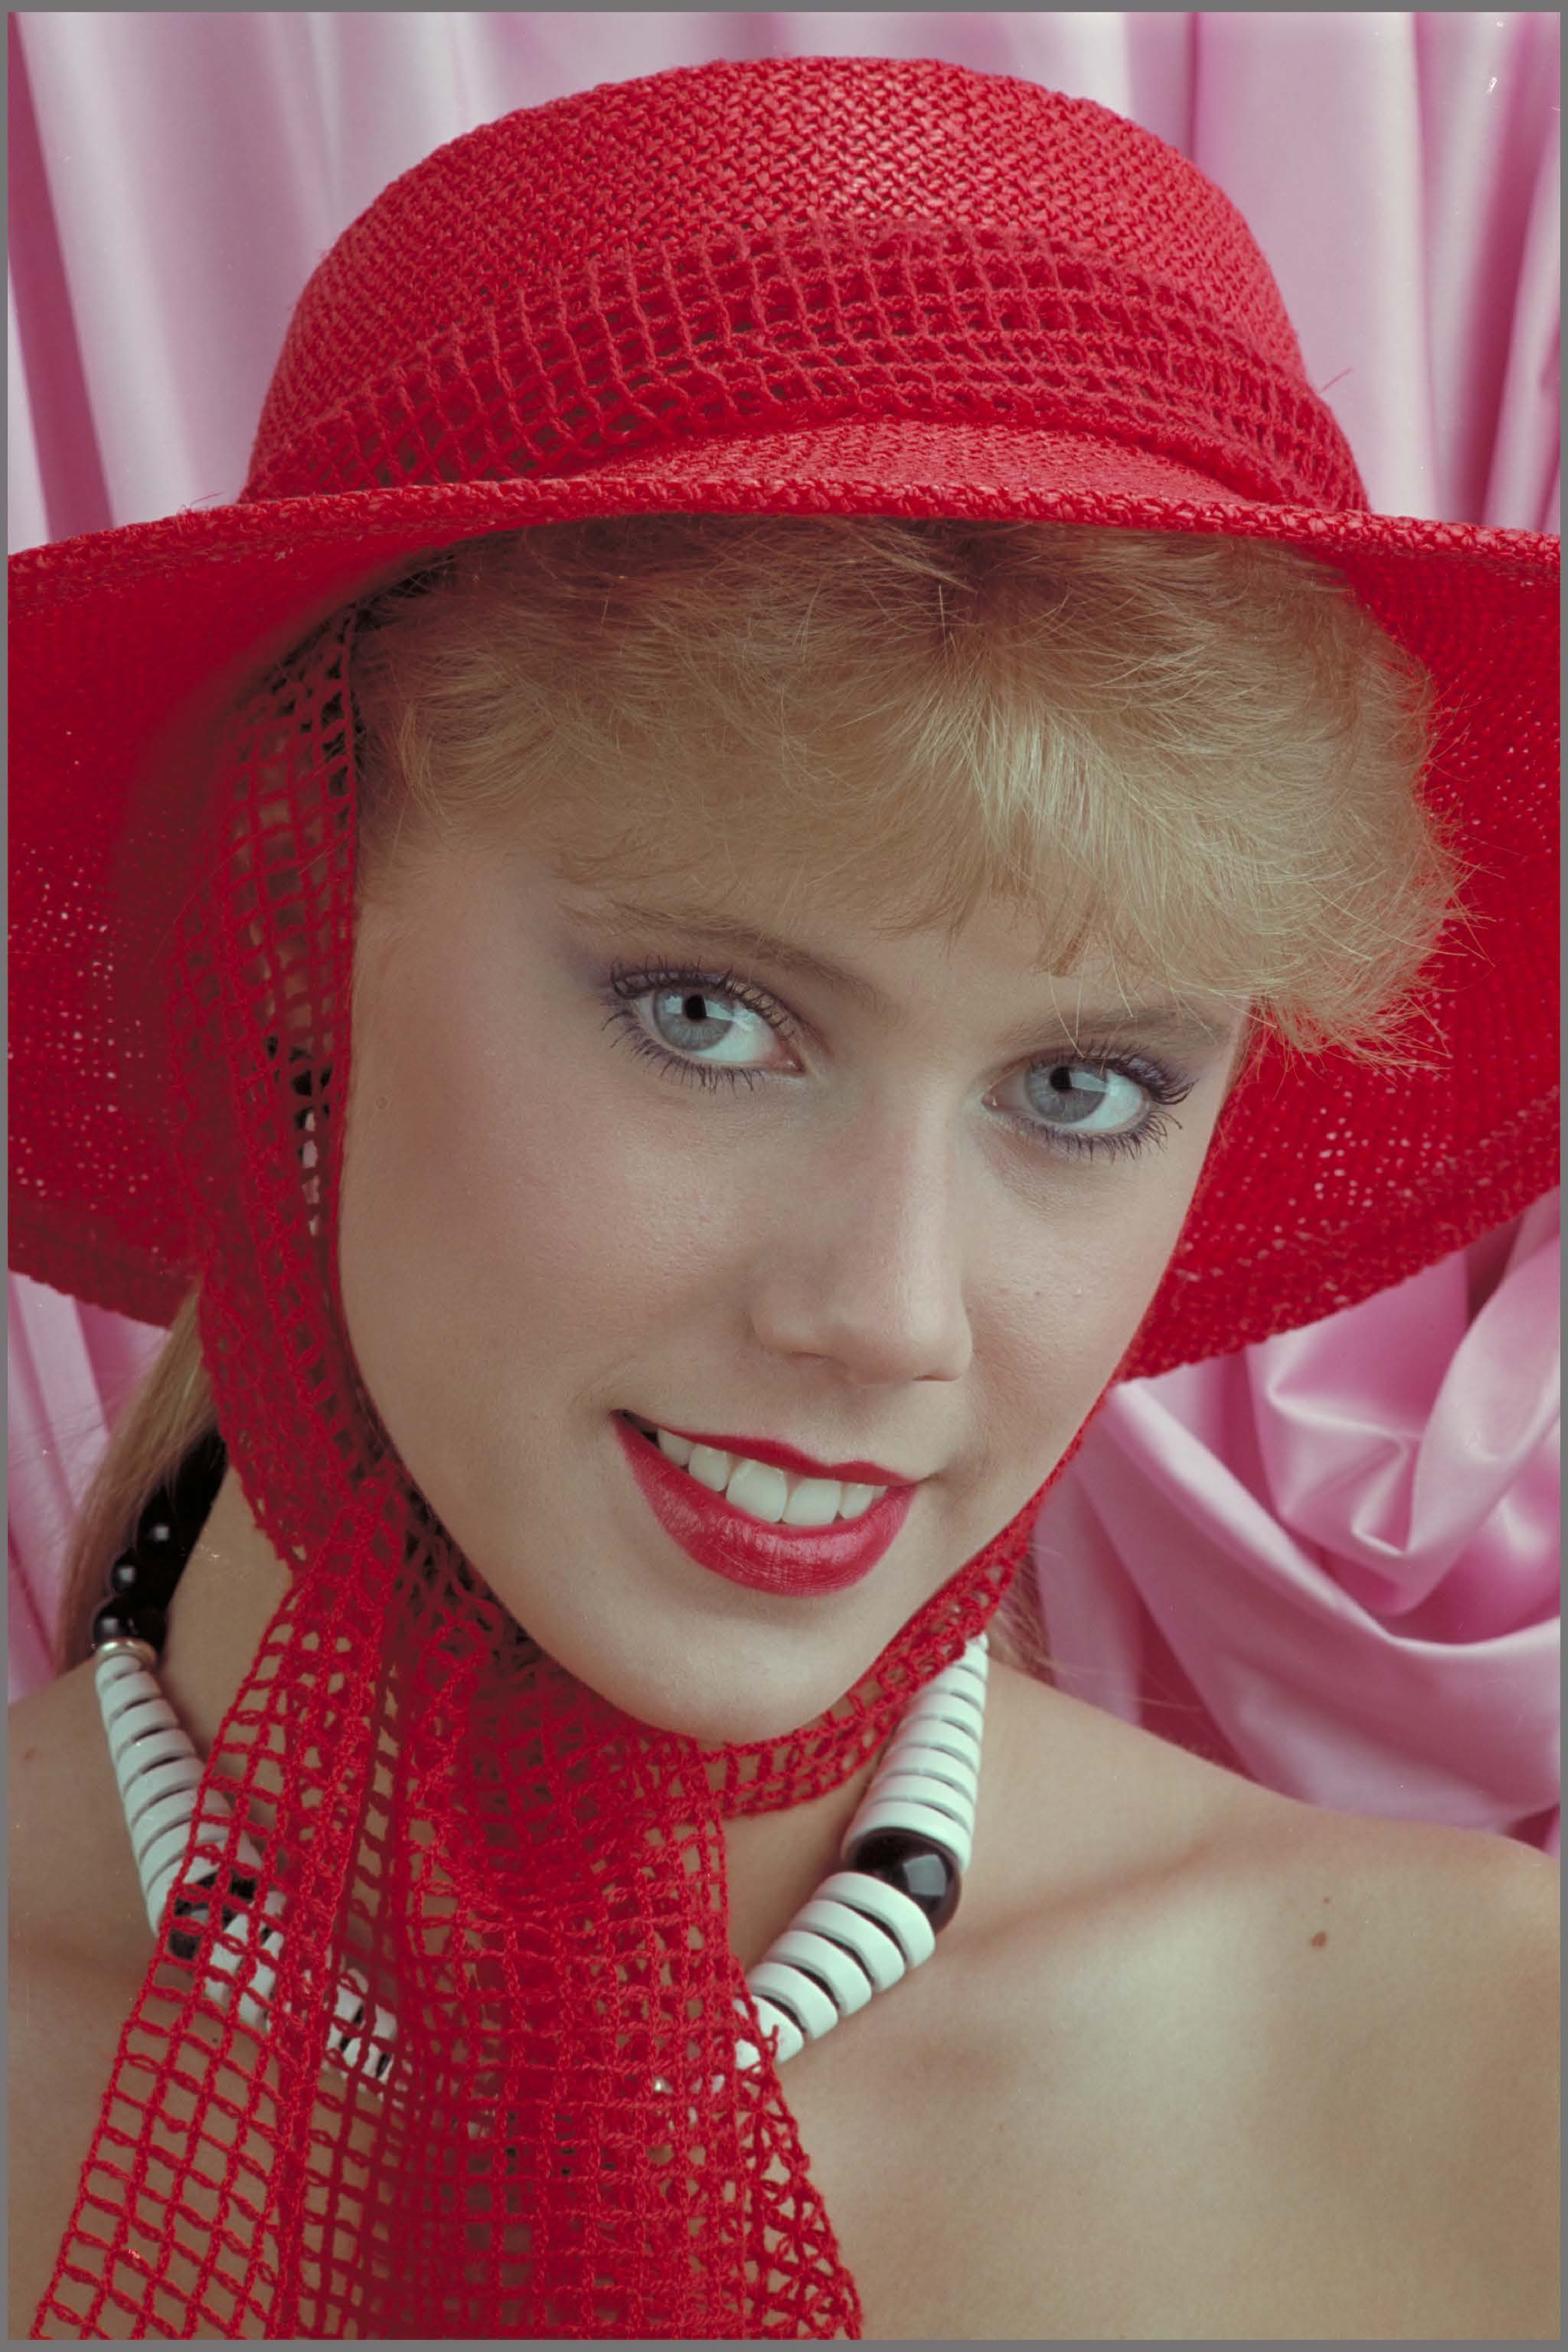
\includegraphics[width=\textwidth]{Immagini/IMAGES/PNG_IMG0004.pdf}
        \caption{Originale}
        \label{fig:OriginalJPEG}
    \end{subfigure}
    \hspace*{1.5cm}
    \begin{subfigure}[]{0.3\textwidth}
        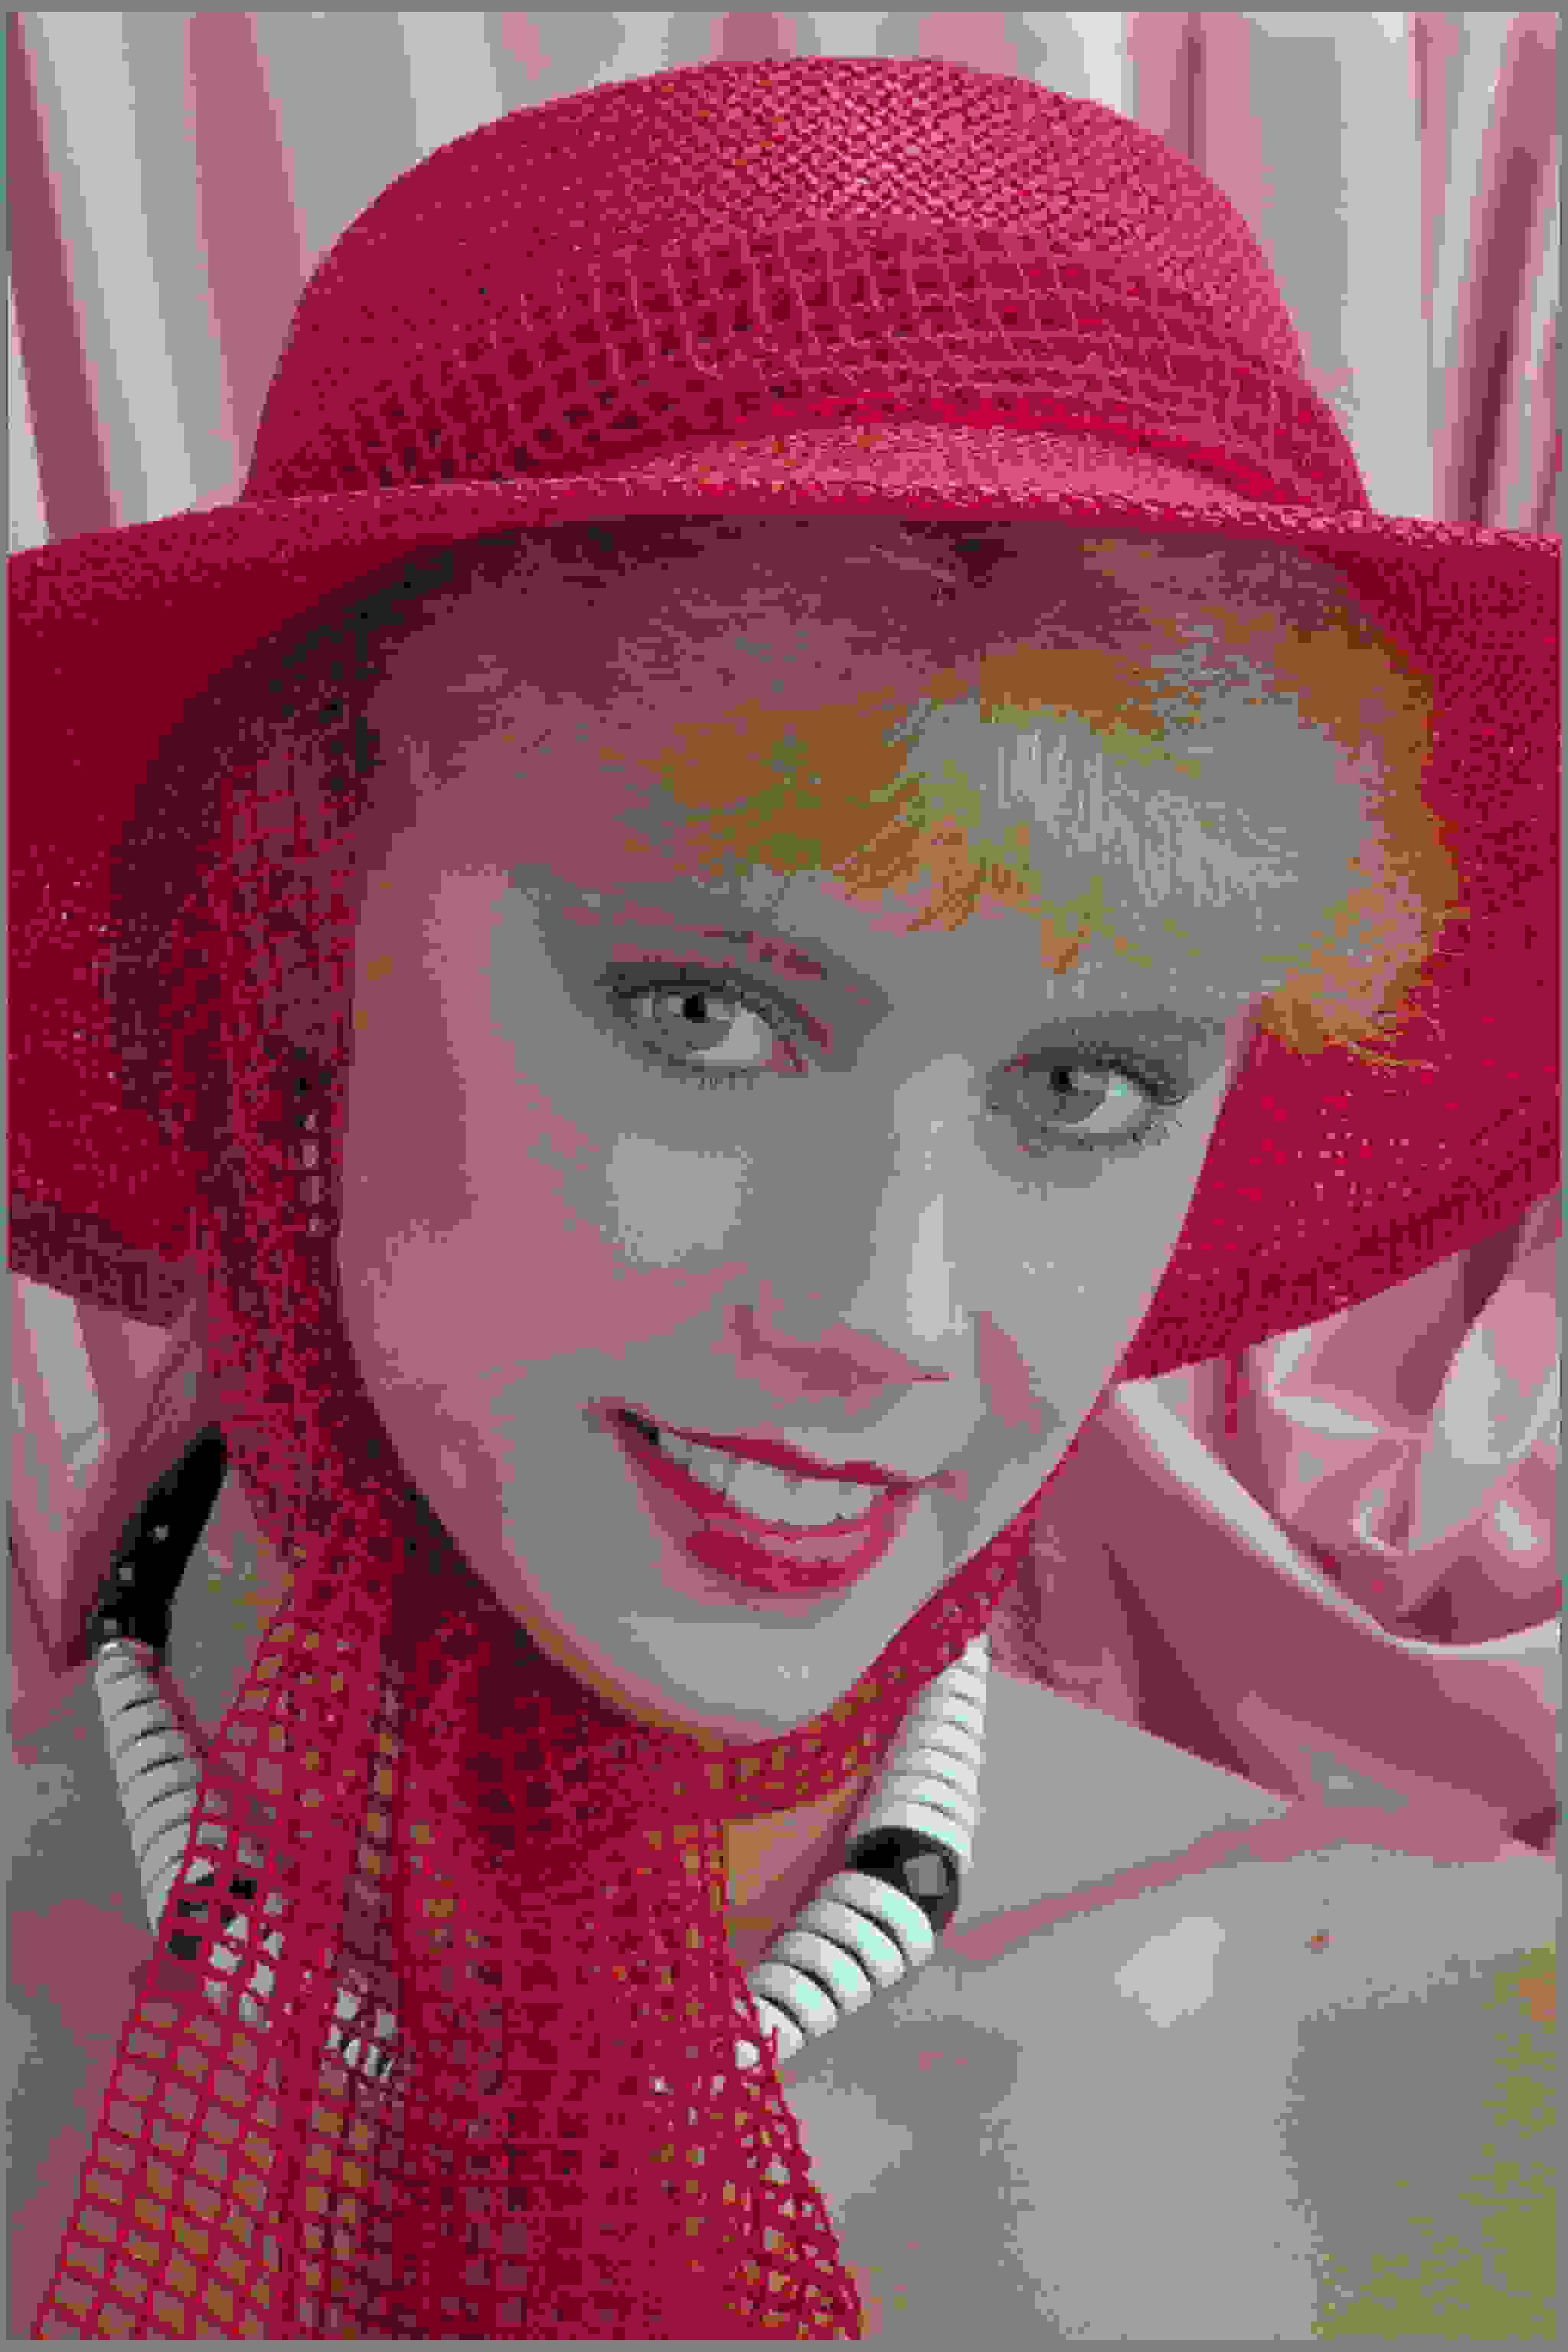
\includegraphics[width=\textwidth]{Immagini/IMAGES/JPEG_1_IMG0004.pdf}
        \caption{JPEG}
        \label{fig:CompressedJPEG}
    \end{subfigure}
    \caption{Confronto PNG con JPEG a 0.167 bpp}
    \label{fig:CompressionJPEG}
\end{figure}

\begin{figure}[h!]
    \centering
    \begin{subfigure}[]{0.3\textwidth}
        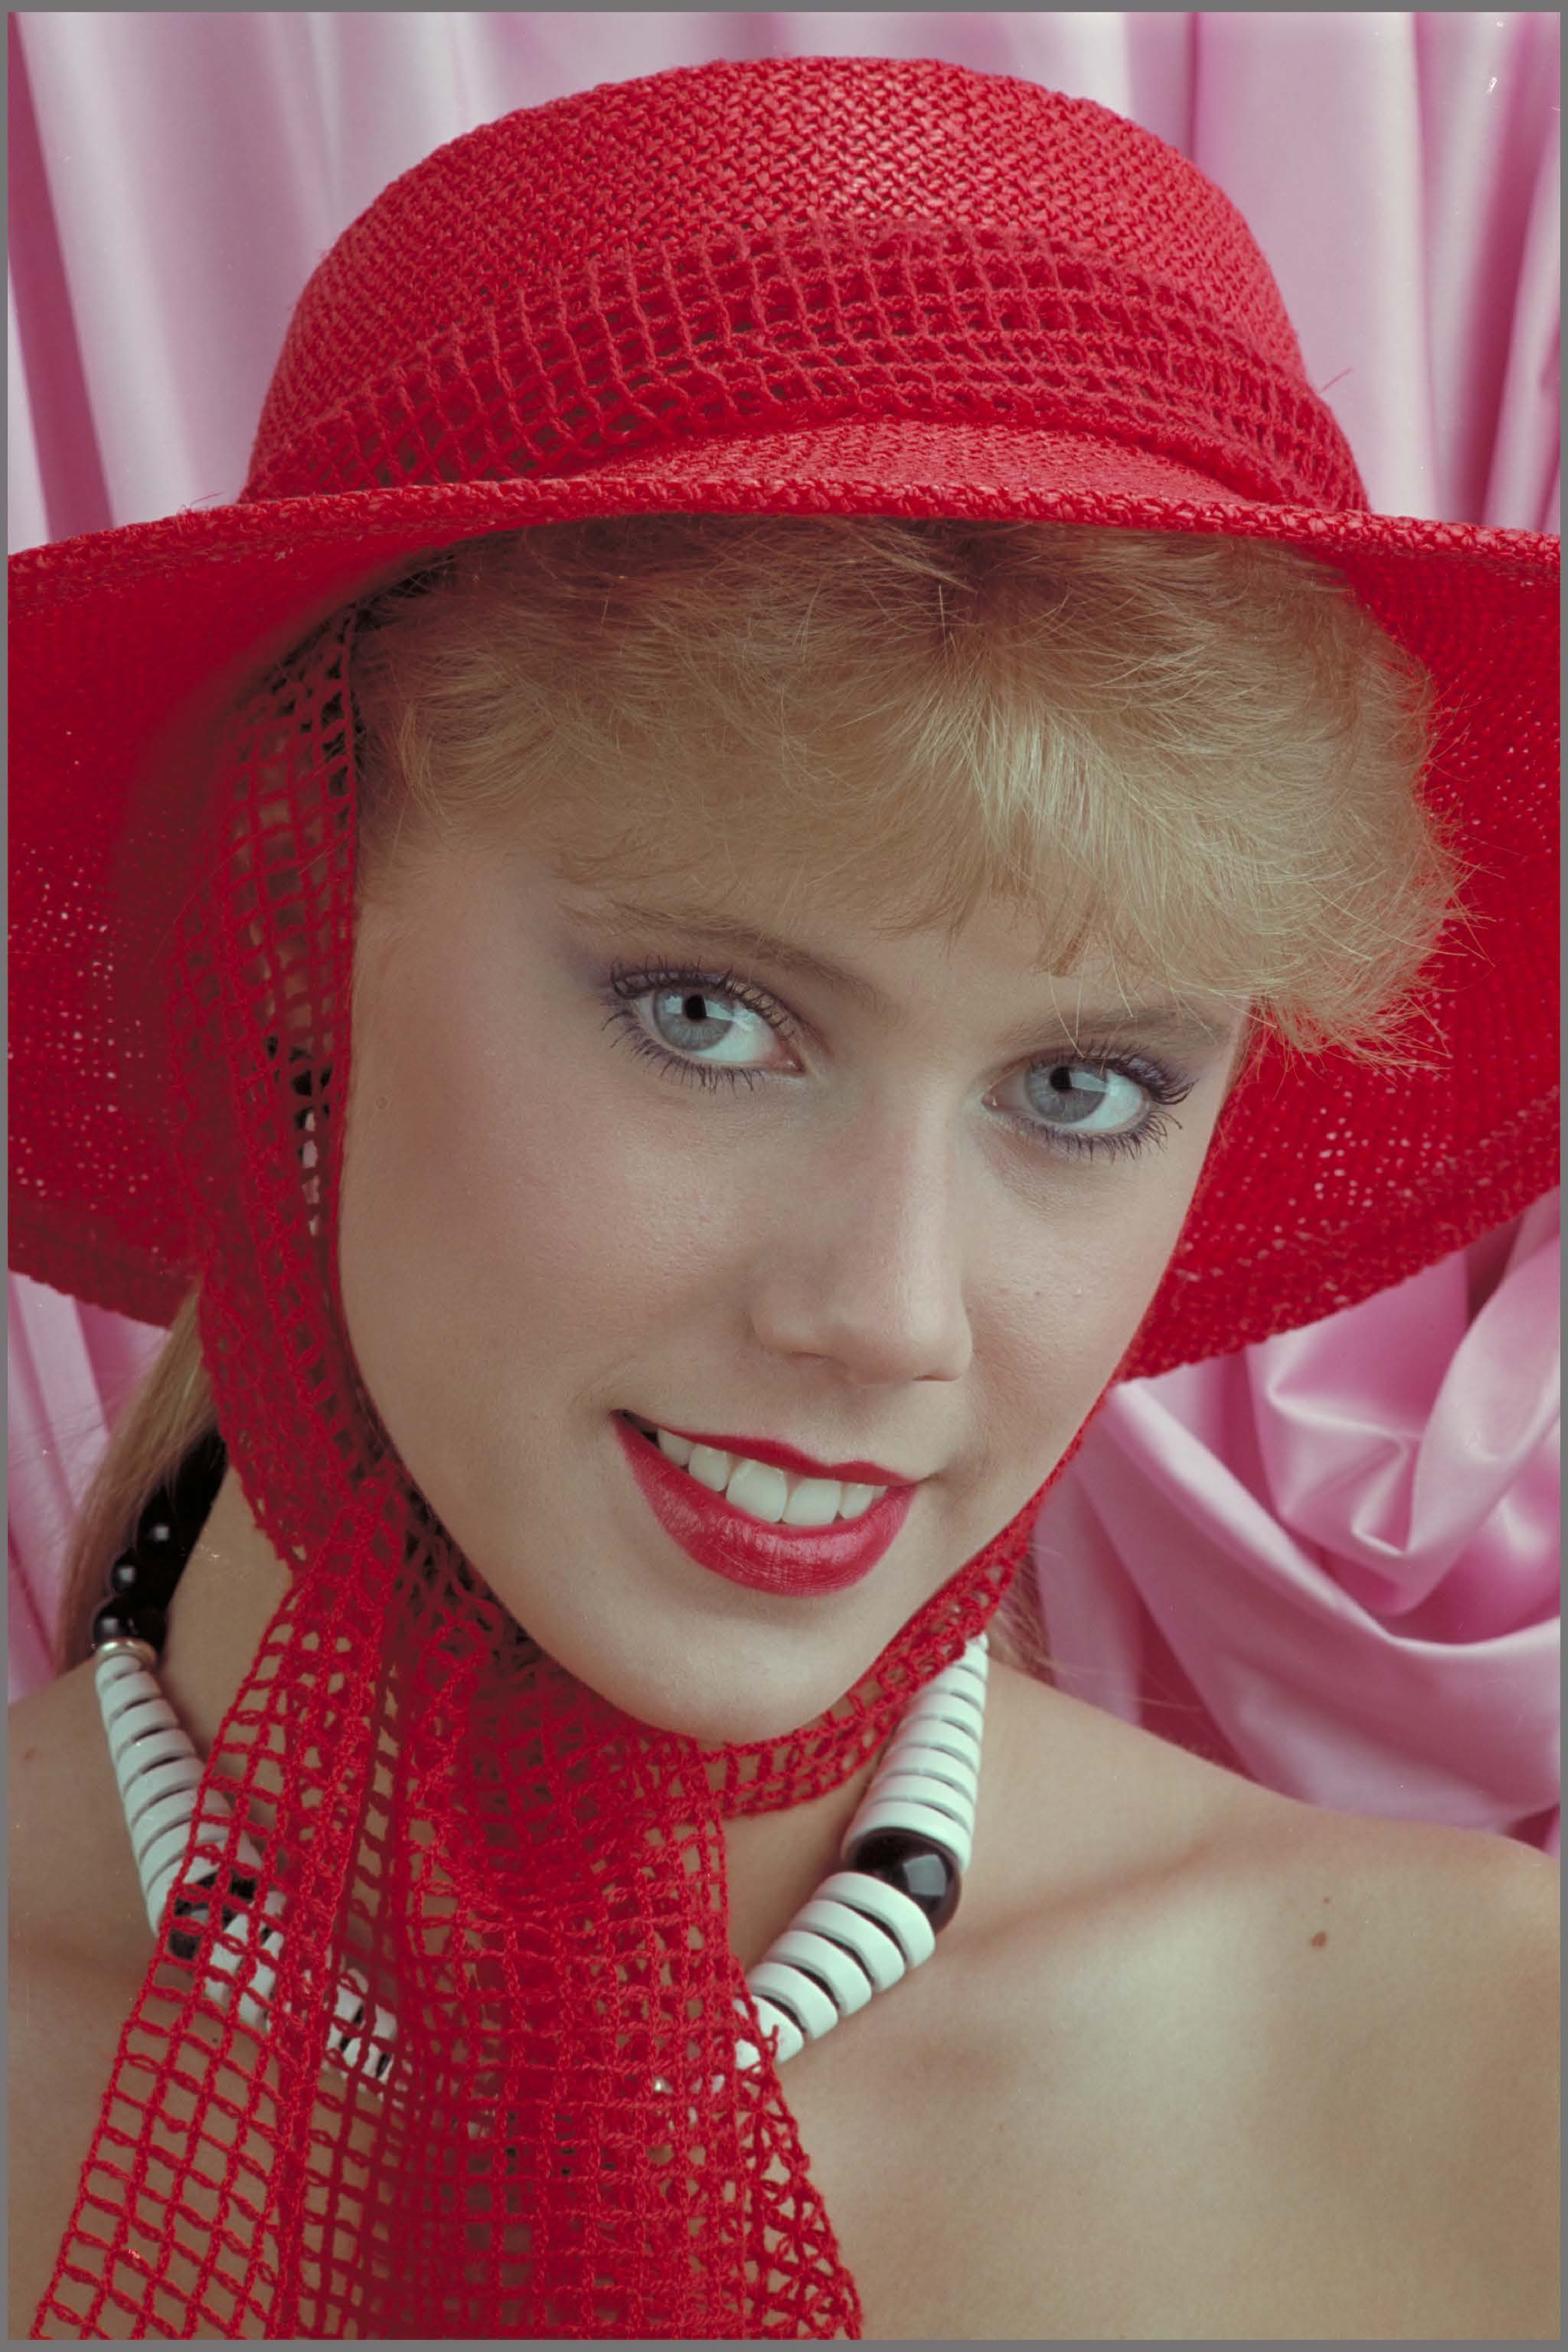
\includegraphics[width=\textwidth]{Immagini/IMAGES/PNG_IMG0004.pdf}
        \caption{Originale}
        \label{fig:OriginalJPEG2000}
    \end{subfigure}
    \hspace*{1.5cm}
    \begin{subfigure}[]{0.3\textwidth}
        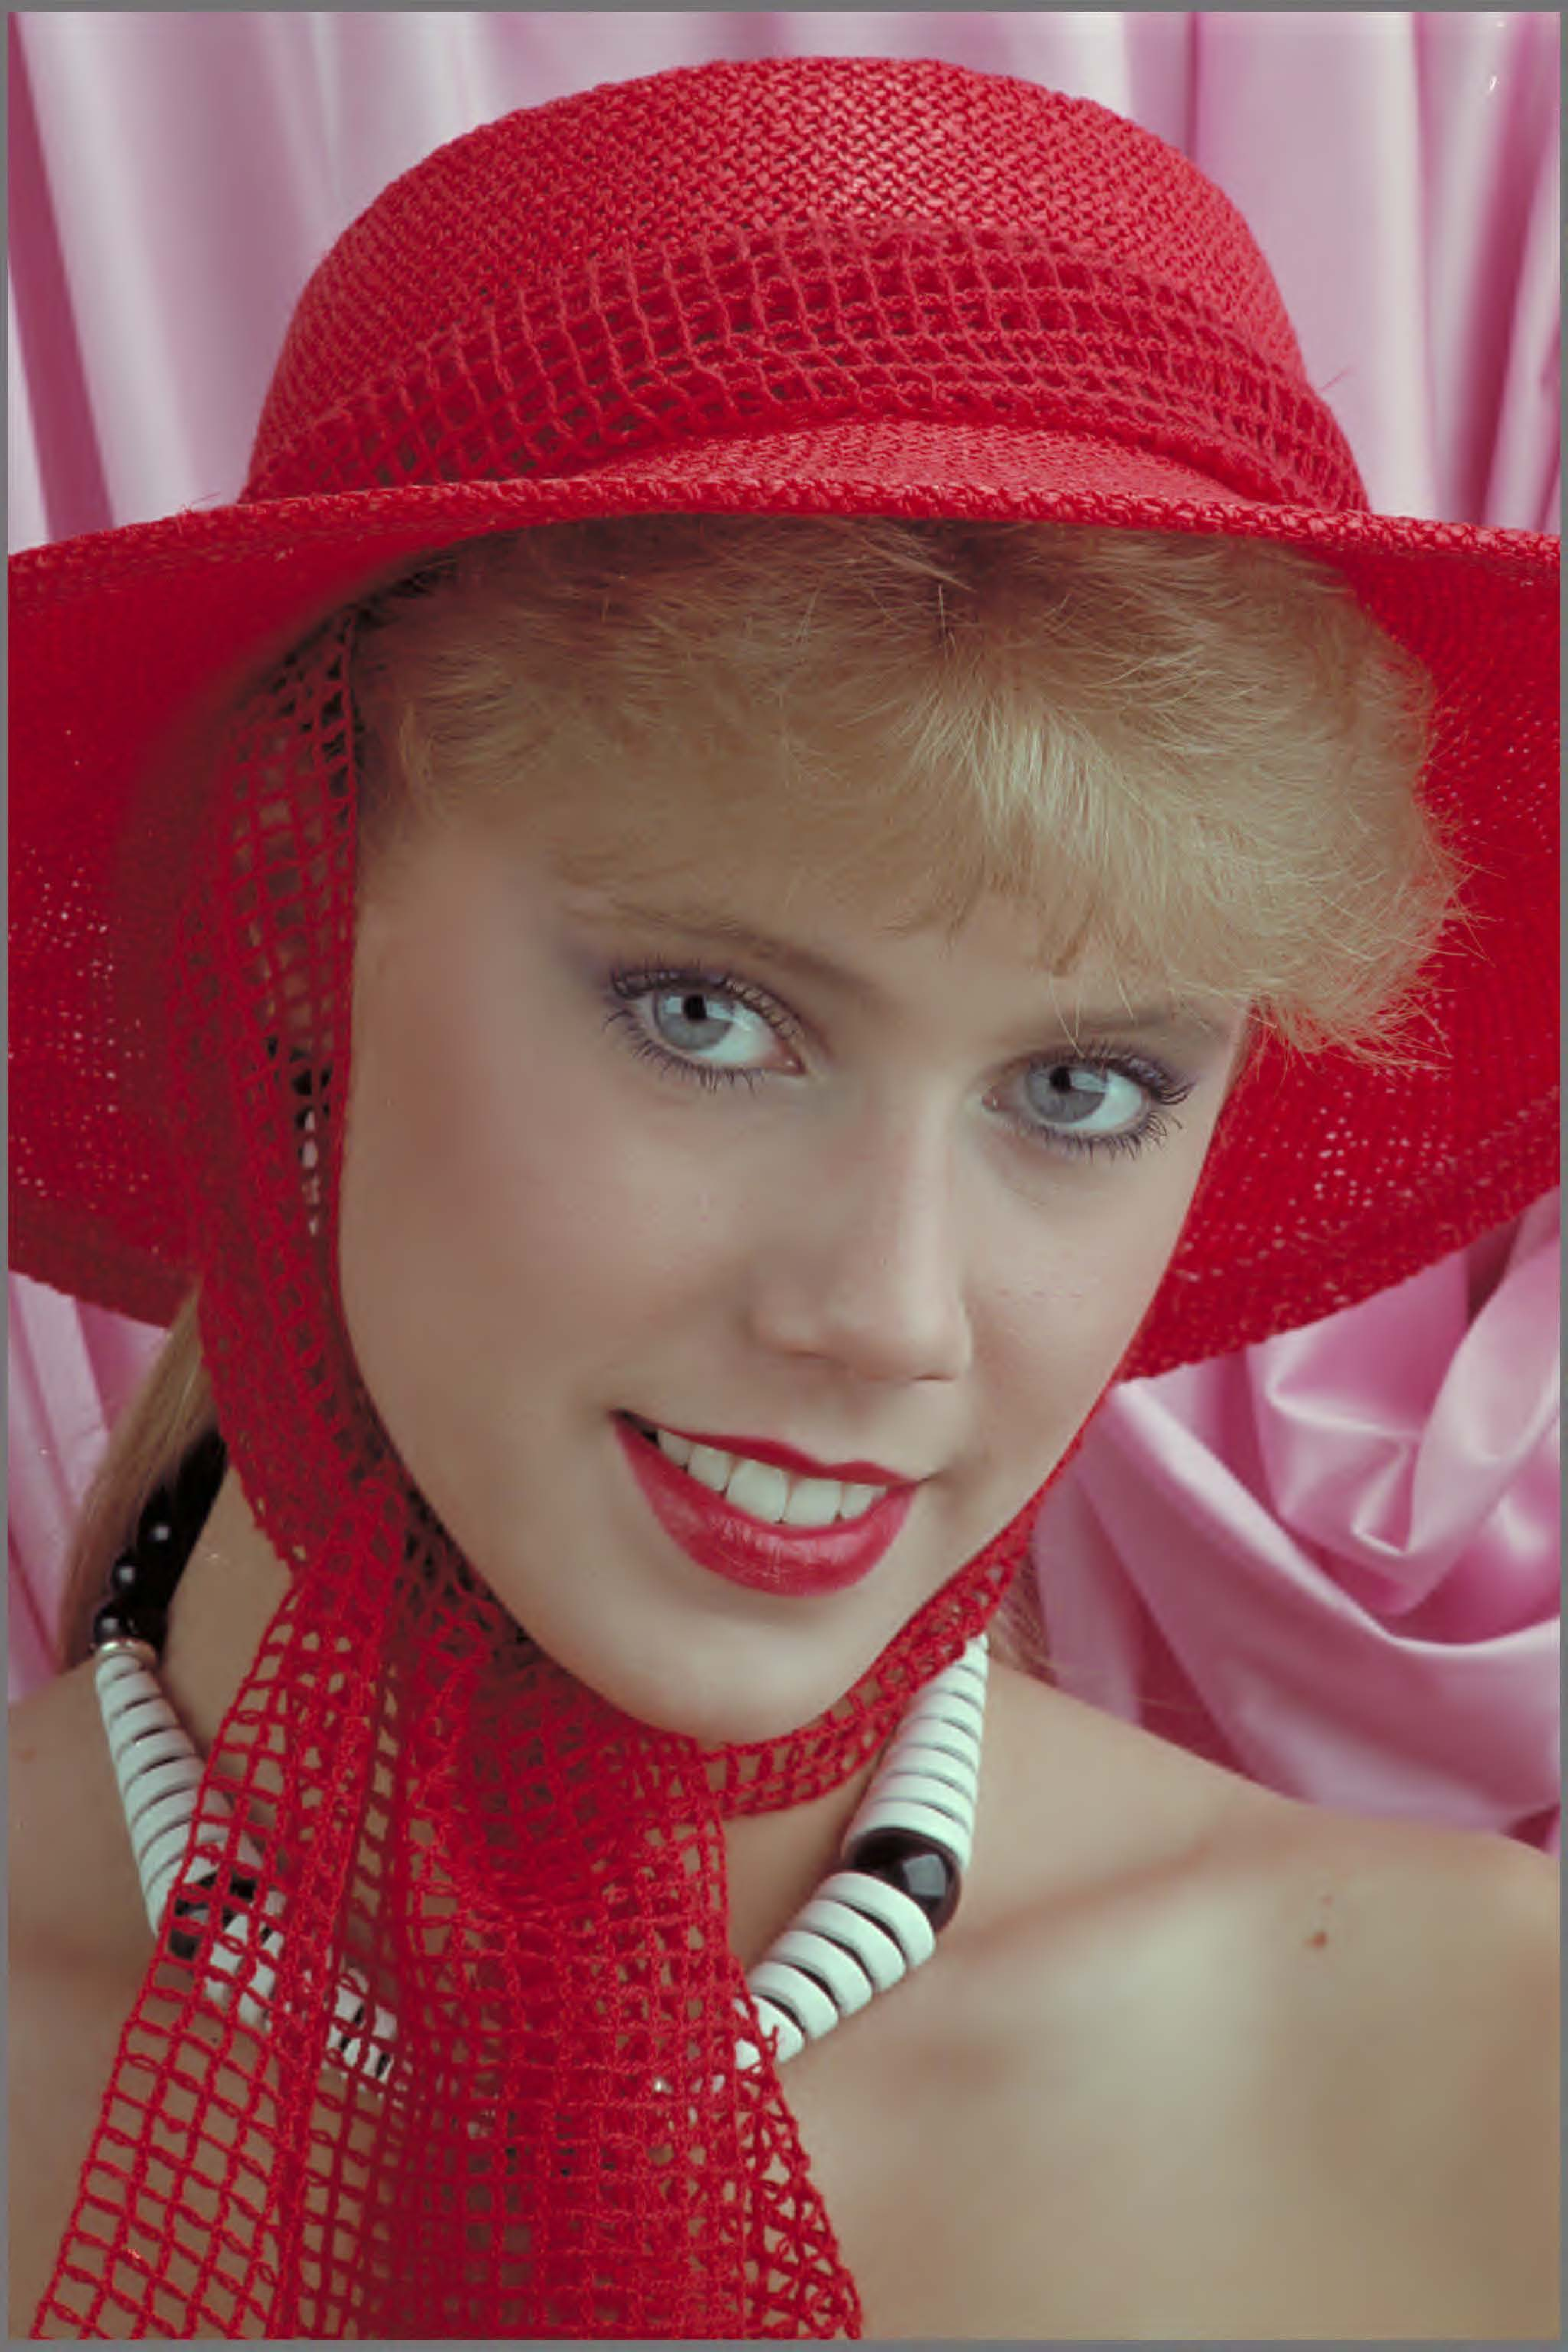
\includegraphics[width=\textwidth]{Immagini/IMAGES/JPEG2000_2_IMG0004.pdf}
        \caption{JPEG2000}
        \label{fig:CompressedJPEG2000}
    \end{subfigure}
    \caption{Confronto PNG con JPEG2000 a 0.171 bpp}
    \label{fig:CompressionJPEG2000}
\end{figure}

\begin{figure}[h!]
    \centering
    \begin{subfigure}[]{0.3\textwidth}
        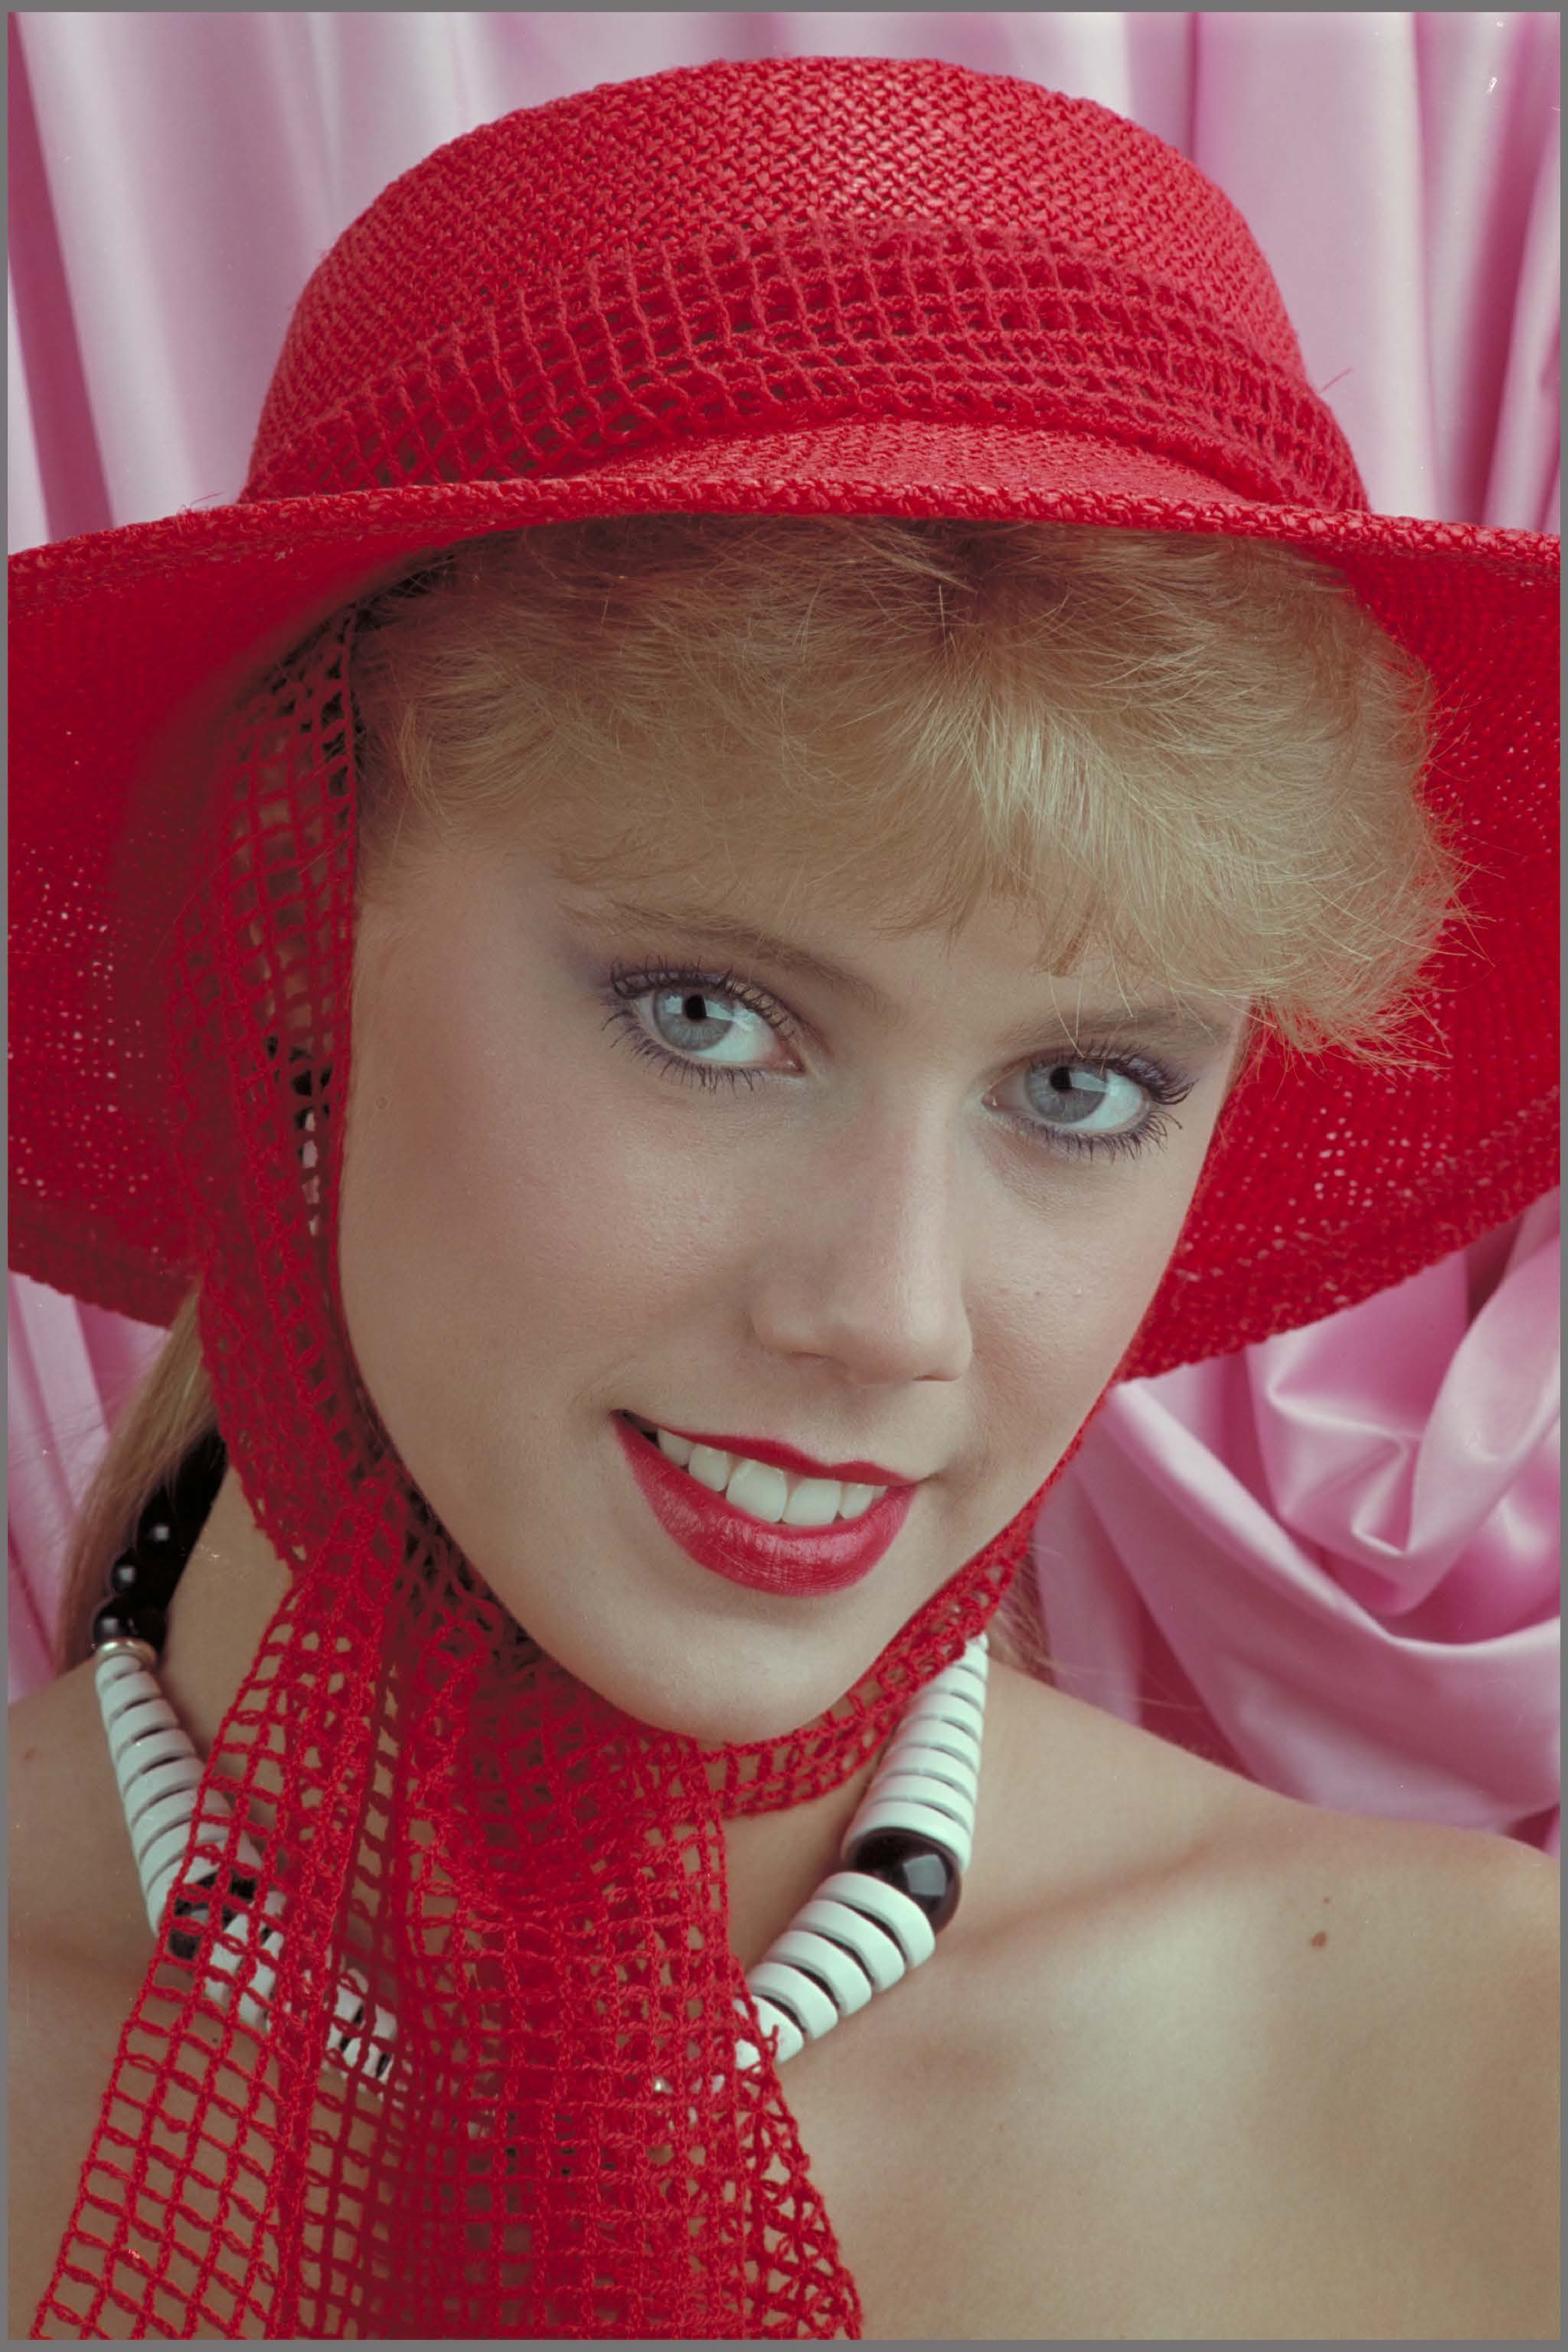
\includegraphics[width=\textwidth]{Immagini/IMAGES/PNG_IMG0004.pdf}
        \caption{Originale}
        \label{fig:OriginalBPG}
    \end{subfigure}
    \hspace*{1.5cm}
    \begin{subfigure}[]{0.3\textwidth}
        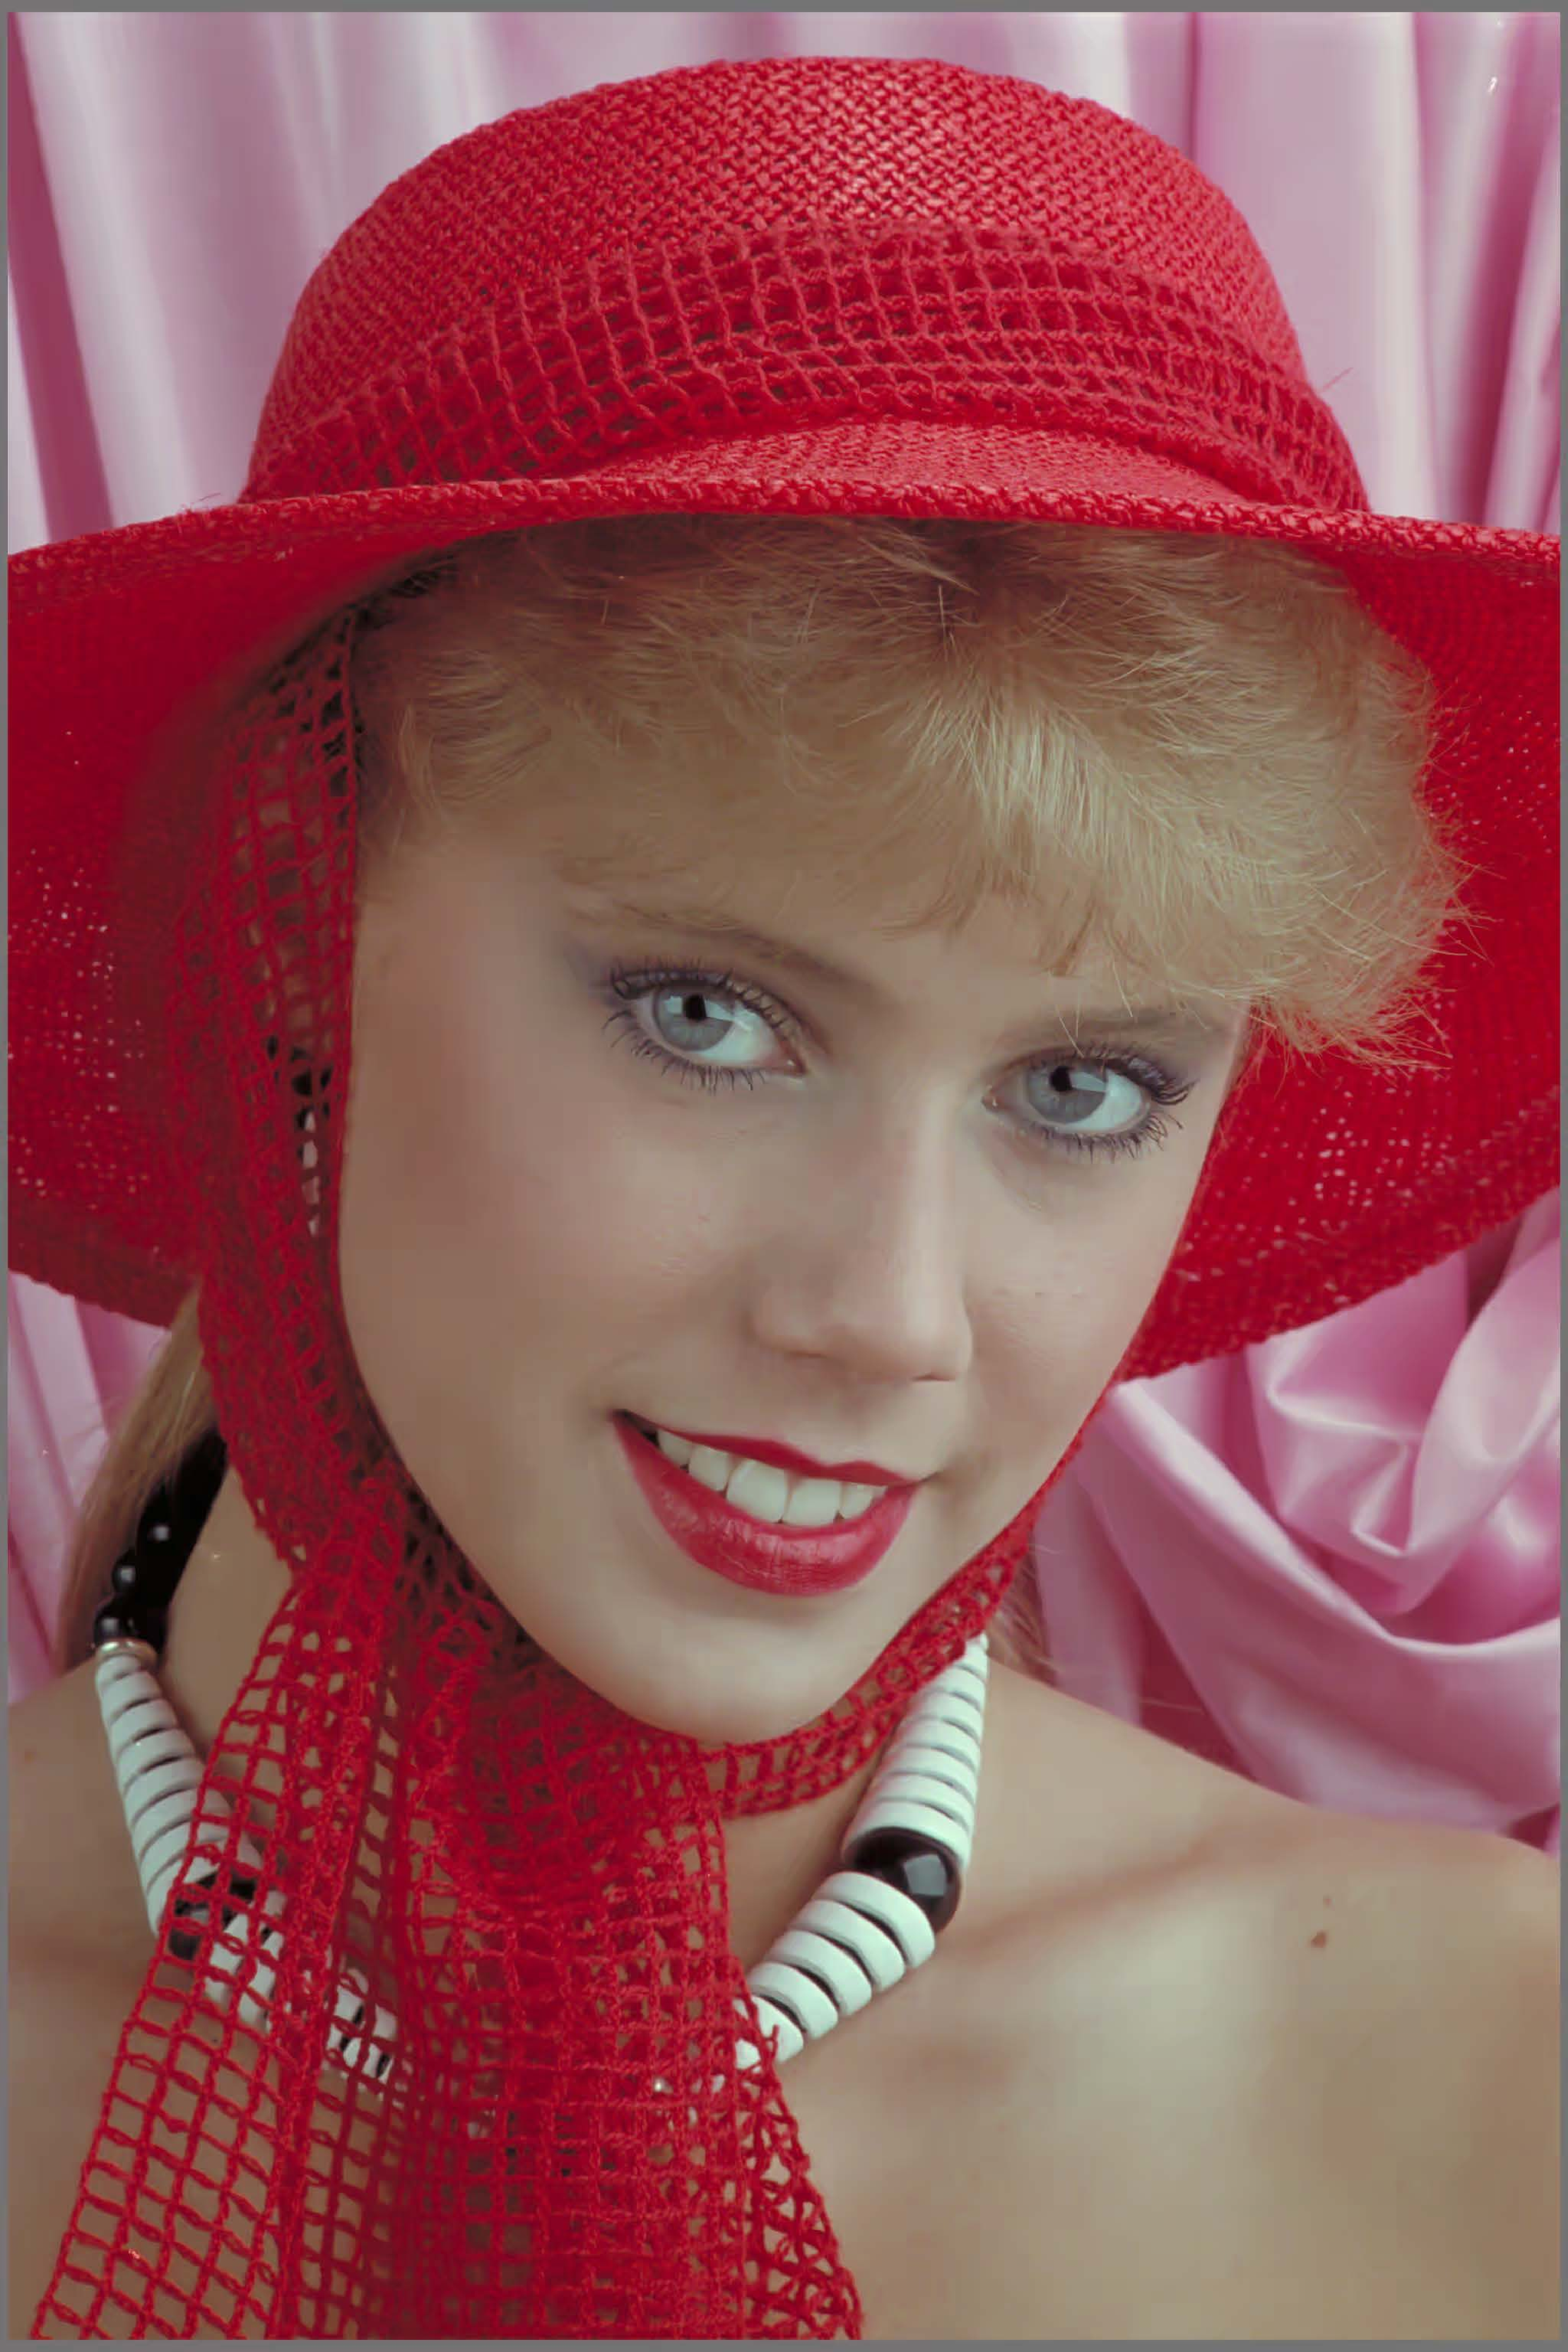
\includegraphics[width=\textwidth]{Immagini/IMAGES/BPG_3_IMG0004.pdf}
        \caption{BPG}
        \label{fig:CompressedBPG}
    \end{subfigure}
    \caption{Confronto PNG con BPG a 0.156 bpp}
    \label{fig:CompressionBPG}
\end{figure}

\begin{figure}[h!]
    \centering
    \begin{subfigure}[]{0.3\textwidth}
        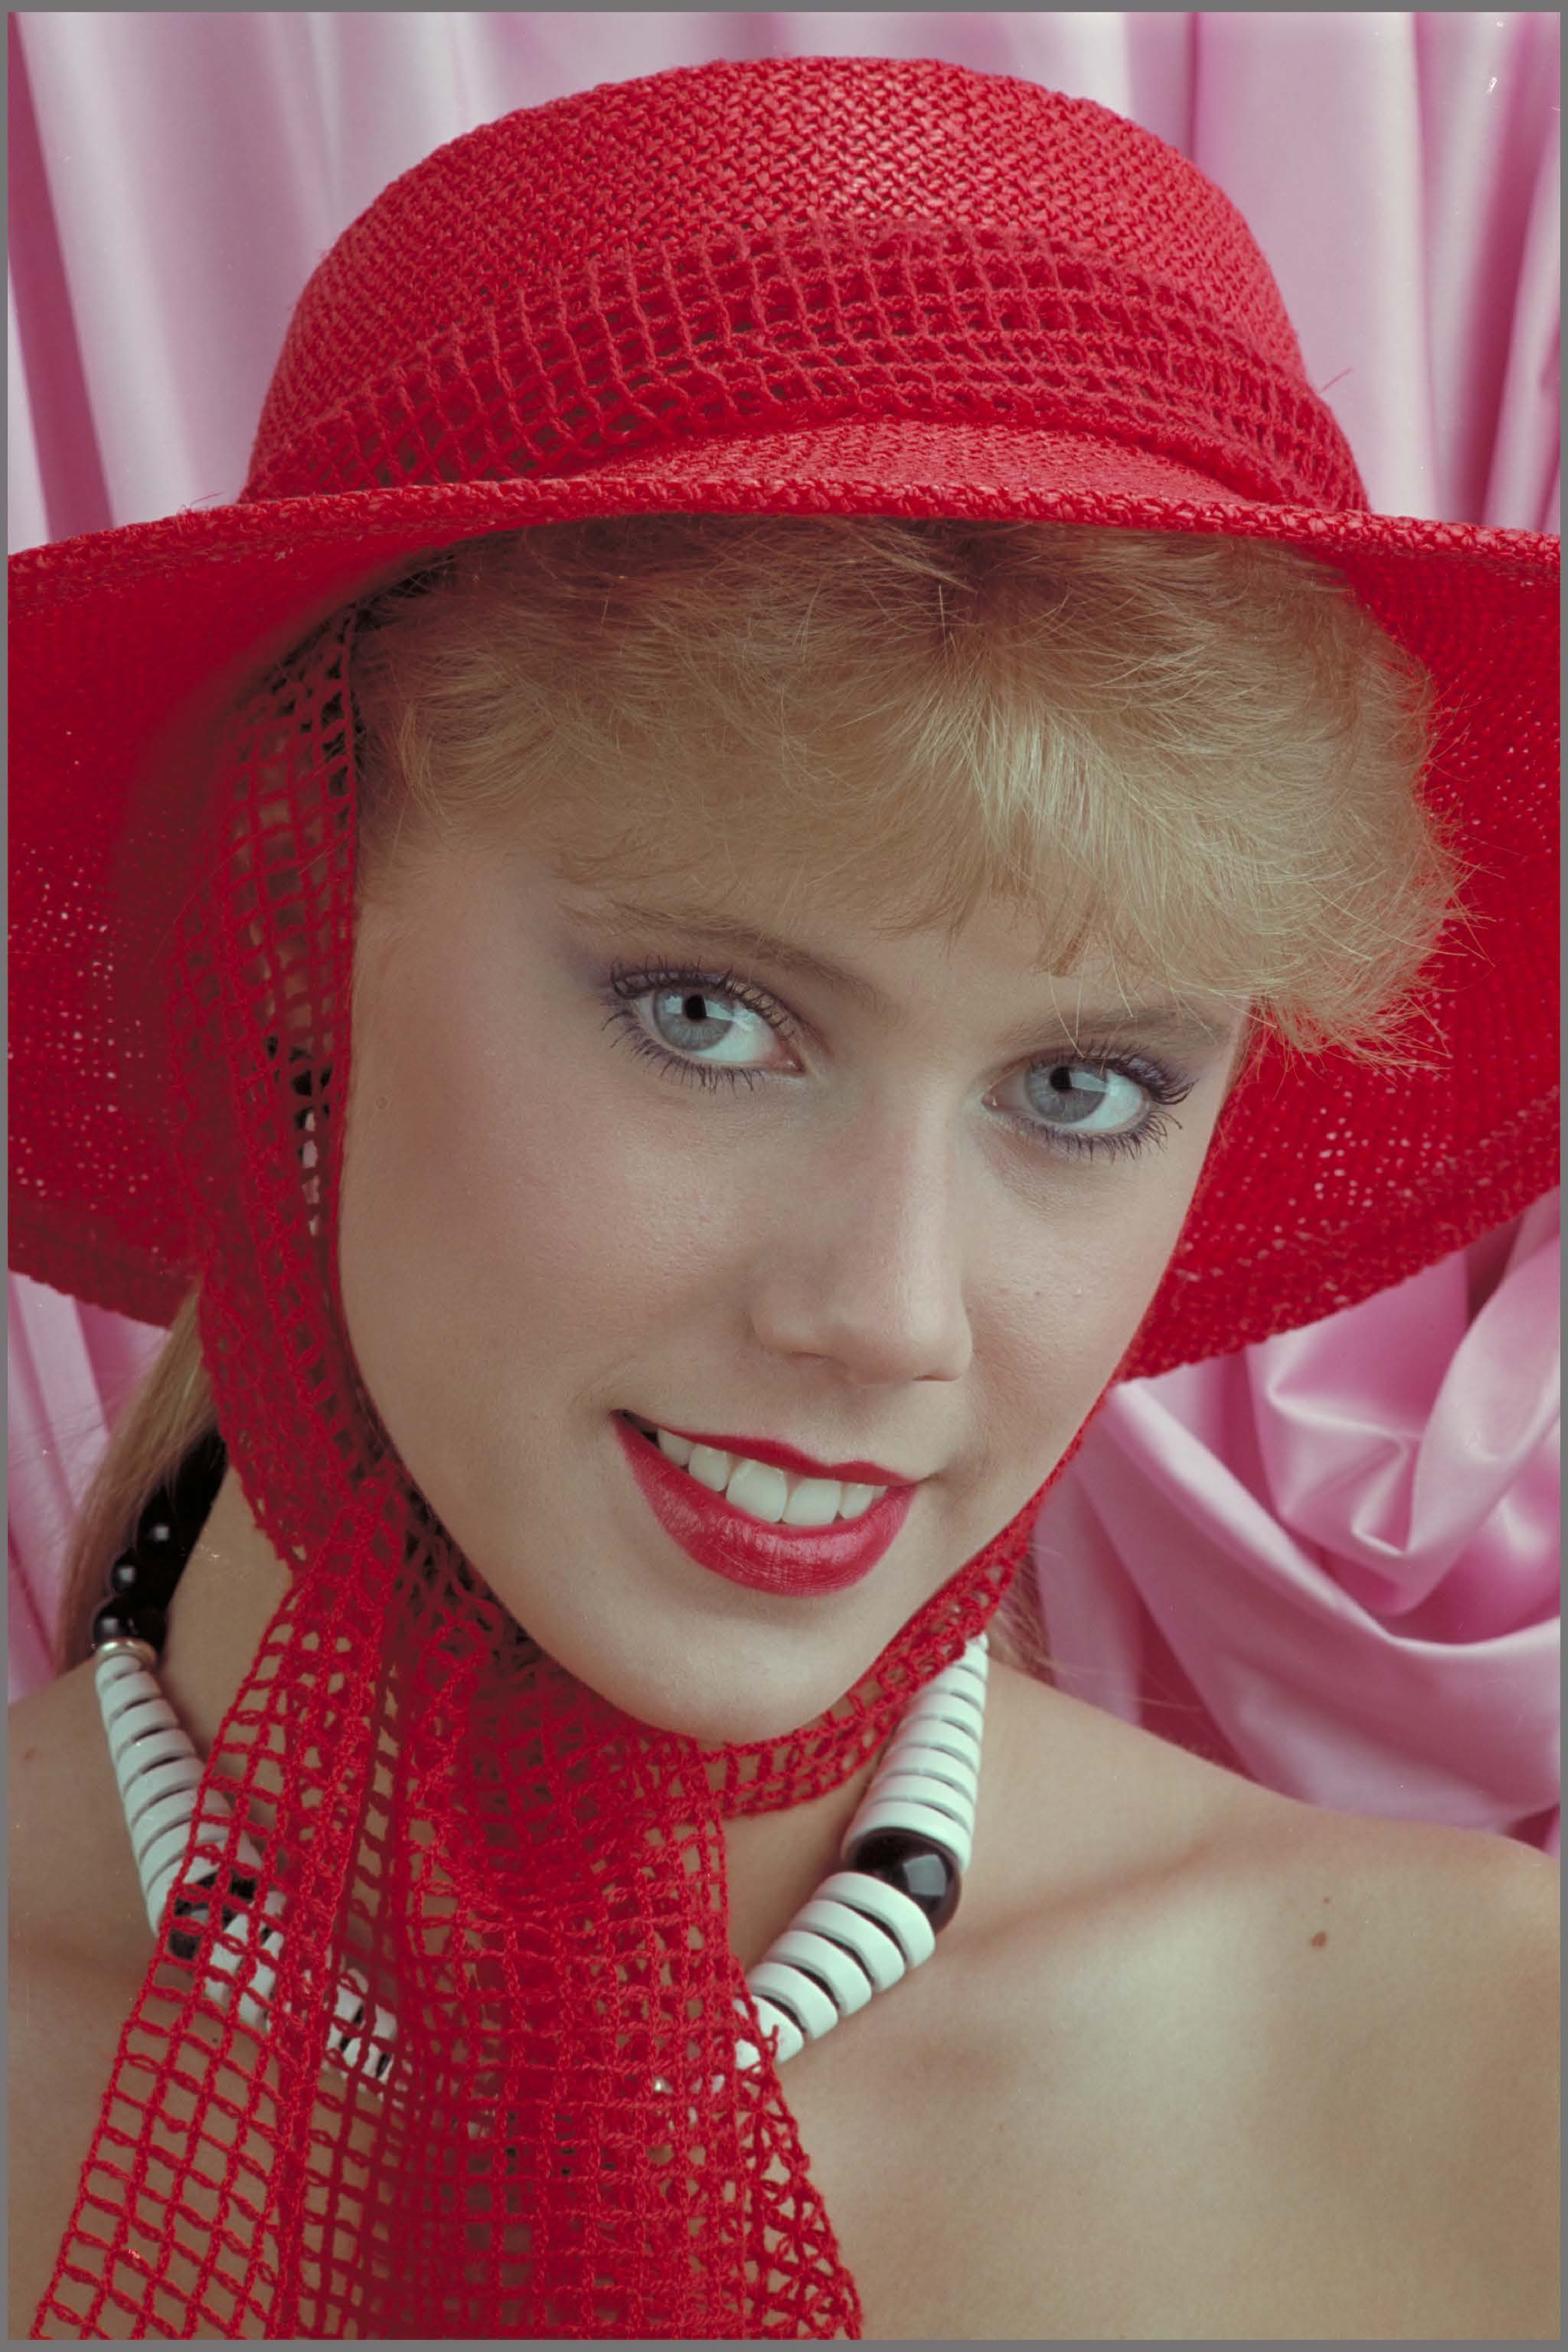
\includegraphics[width=\textwidth]{Immagini/IMAGES/PNG_IMG0004.pdf}
        \caption{Originale}
        \label{fig:OriginalVVC}
    \end{subfigure}
    \hspace*{1.5cm}
    \begin{subfigure}[]{0.3\textwidth}
        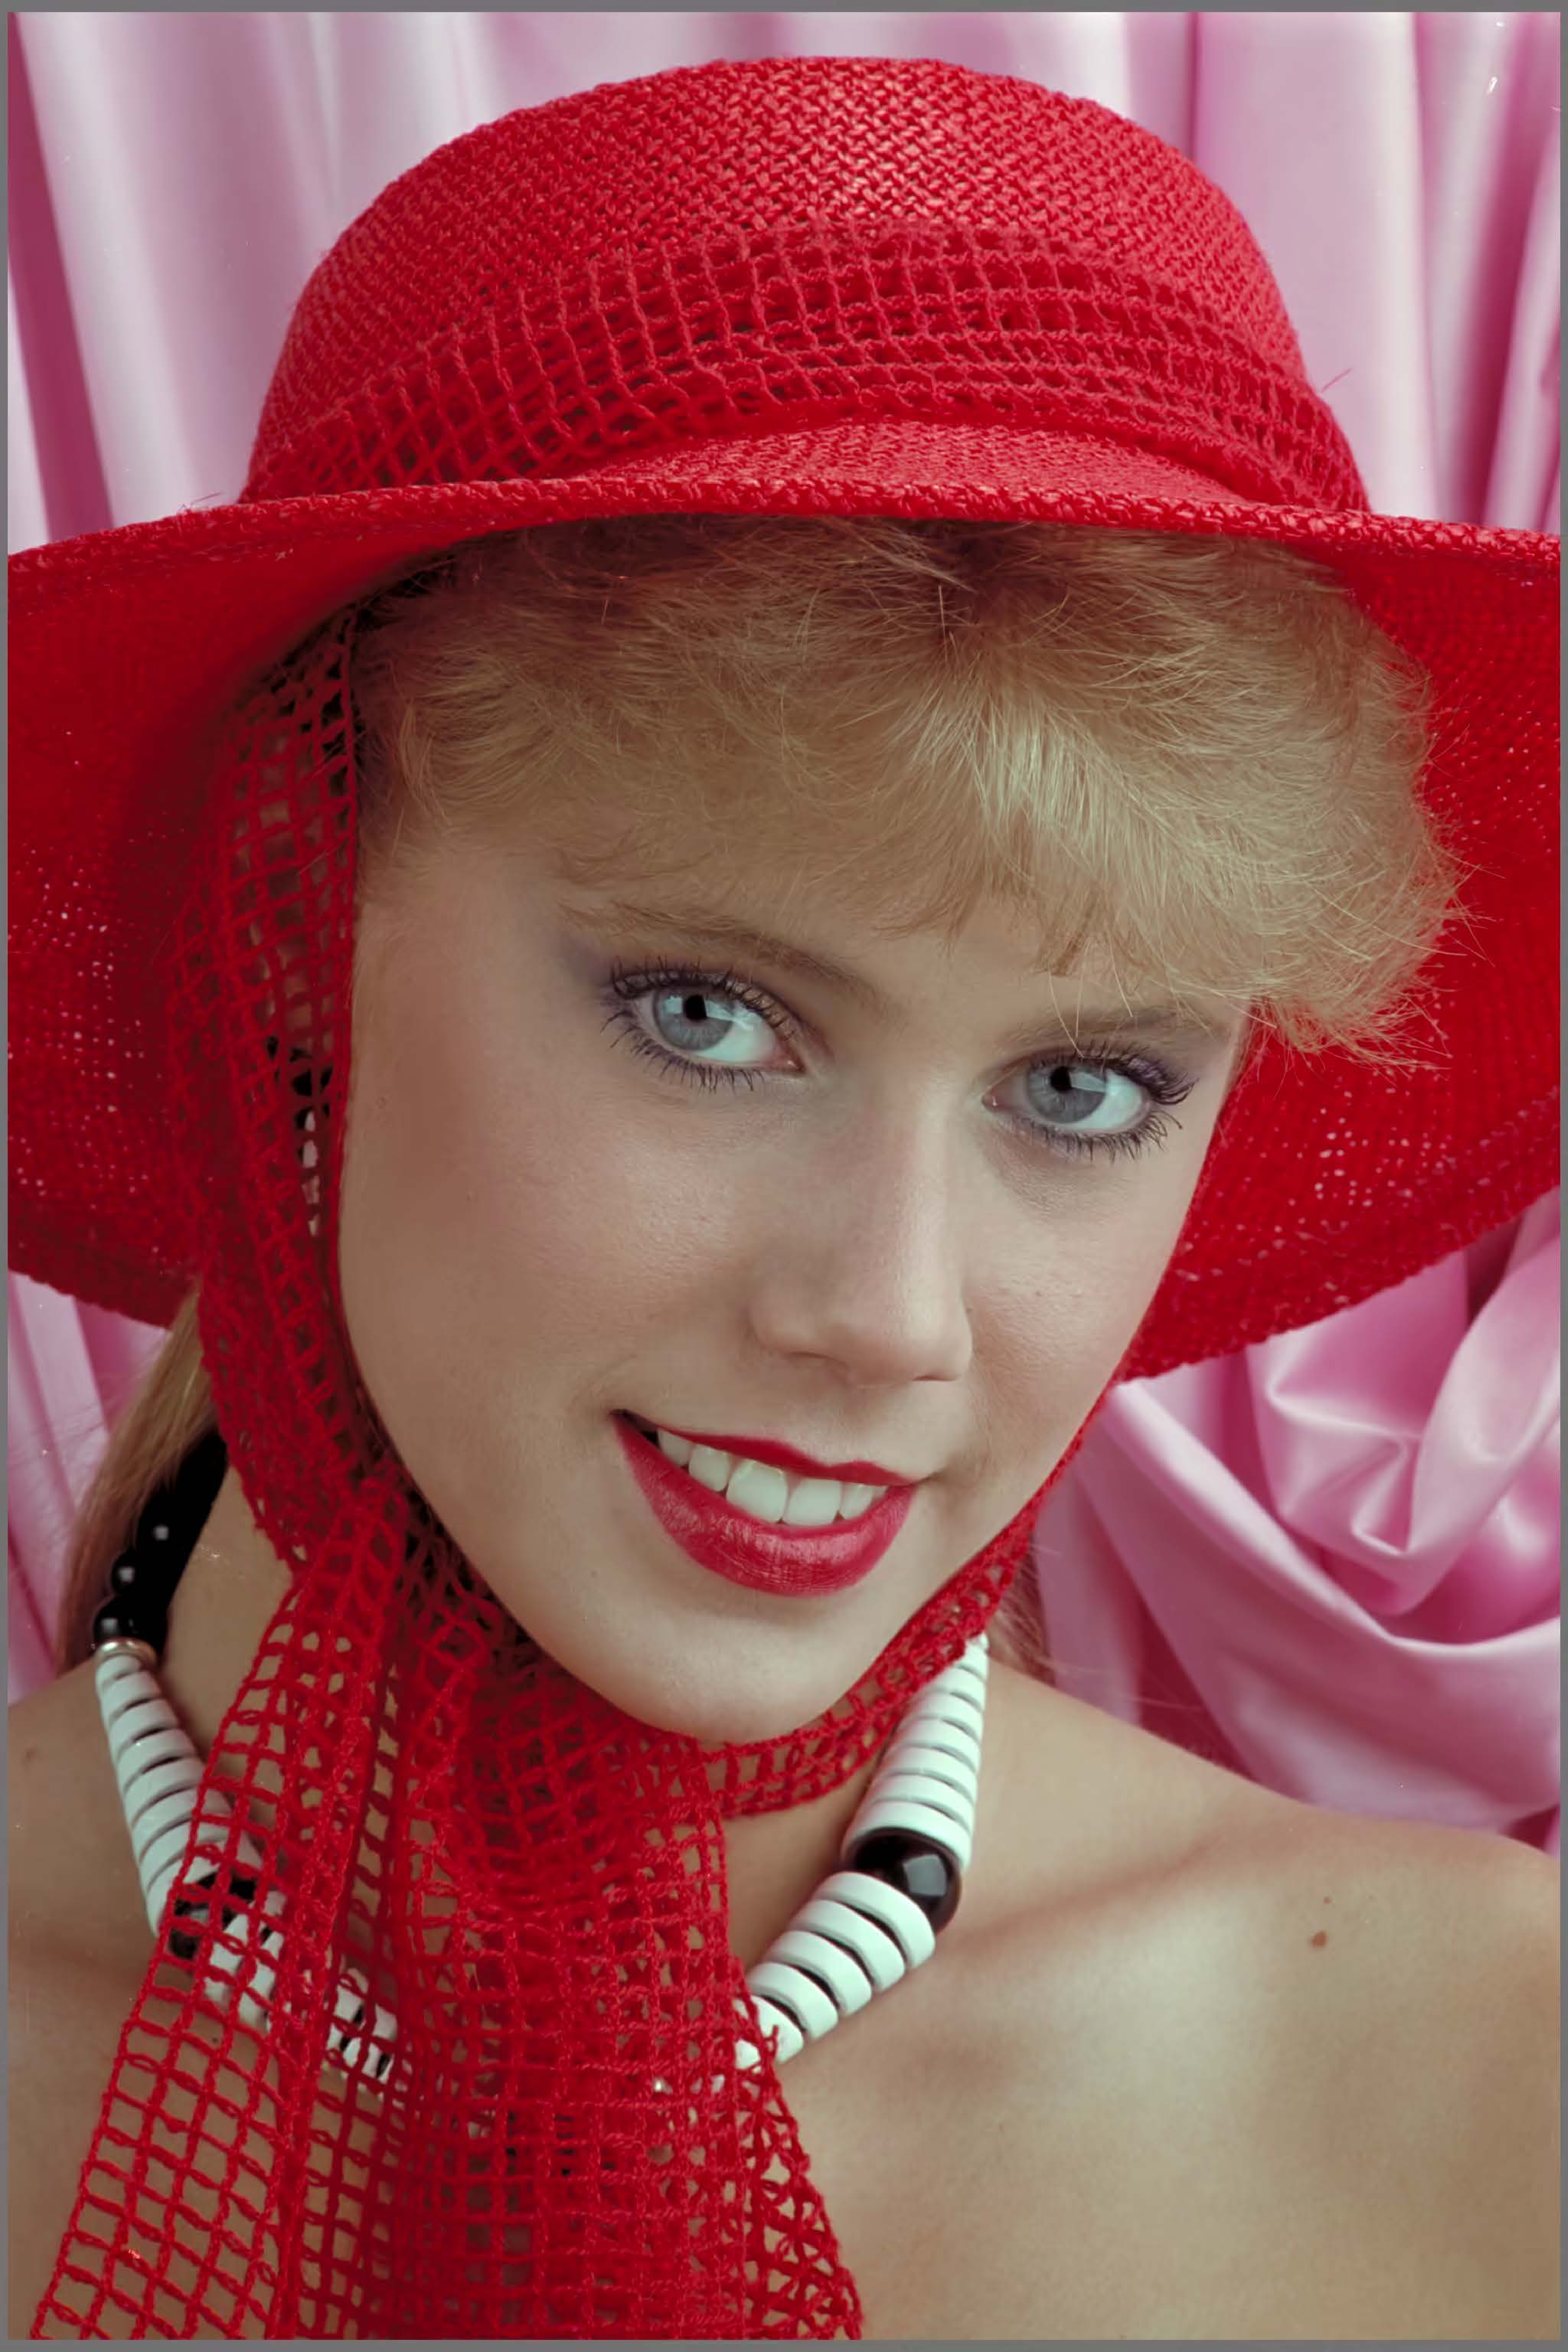
\includegraphics[width=\textwidth]{Immagini/IMAGES/VVC_2_IMG0004.pdf}
        \caption{VVC}
        \label{fig:CompressedVVC}
    \end{subfigure}
    \caption{Confronto PNG con VVC a 0.144 bpp}
    \label{fig:CompressionVVC}
\end{figure}